\chapter{Our Distillation Framework for Pixel-Space Diffusion}
\label{chap:framework}

% ============================================================
\section{Framework Overview and Motivation}
\label{sec:framework_overview}
% ============================================================

The prevailing paradigm of knowledge distillation applied to diffusion models has been almost exclusively concerned with \emph{sampling acceleration}: given a fully trained teacher, a student is trained to reproduce the teacher's output in fewer denoising steps, thereby reducing the number of function evaluations (NFE) at inference time \cite{salimans2022progressive, song2023consistency, luo2023lcm}. While this line of work is practically valuable, it addresses a fundamentally different objective than the one pursued in this thesis. Sampling-acceleration methods do not alter the capacity or representational quality of the student model; a student that converges under such a scheme simply learns to approximate the teacher's multi-step trajectory in fewer steps, but it cannot surpass the teacher's generative quality ceiling at a fixed NFE. Our goal is orthogonal: we seek to \emph{improve the generative quality} of a smaller JiT model without modifying its inference-time architecture, parameter count, or computational cost. That is, for an identical deployment budget, we aim to produce a strictly higher-quality generative model by leveraging supervision from a larger, pretrained JiT teacher during training. The distillation signal is discarded at inference time; the student runs as a standalone model.

This quality-boosting objective is enabled by a property specific to JiT \cite{li2025jit}: it operates directly in pixel space. Unlike latent diffusion models \cite{rombach2022ldm}, whose denoising trajectories unfold over opaque, high-dimensional latent codes with no direct visual interpretation, JiT's intermediate states at every denoising timestep are actual noisy images — semantically grounded, spatially structured, and directly inspectable. This observability has a concrete consequence for distillation: the internal representations of JiT, including its multi-head self-attention maps and intermediate feature tensors, are dense, spatially coherent, and carry interpretable information about image structure at every point along the denoising trajectory. In latent-space models, by contrast, such intermediate representations encode statistics of an abstract embedding space, and their spatial correspondence to image content is indirect and architecture-dependent. The pixel-space setting thus exposes a richer and more supervisable knowledge structure, making JiT a uniquely suitable backbone for feature-level distillation.

Concretely, this thesis investigates three complementary distillation strategies applied within a unified teacher--student framework. The teacher is a larger, pretrained JiT variant with its weights held frozen throughout training. The student is a smaller JiT variant trained from scratch — or from an informed initialisation — under the combined supervision of the standard flow-matching objective and additional distillation losses derived from the teacher's internal representations. We conduct experiments on two benchmarks at different scales of difficulty: CIFAR-10 \cite{krizhevsky2009cifar}, where the teacher--student pair is JiT-S/2 (48.2M parameters) and JiT-T/2 (16.5M parameters), respectively; and ImageNet-1K \cite{russakovsky2015imagenet}, where the pair is JiT-B/16 (teacher) and JiT-S/16 (student). Full experimental details, training protocols, and quantitative results are reported in Chapter~\ref{chap:experiments}.

The three distillation strategies are as follows. First, the primary methodology is \emph{feature map distillation via ViTKD} (Section~\ref{sec:vitkd}), which transfers knowledge encoded in the intermediate hidden-state tensors of the teacher's transformer blocks. Second, \emph{attention map distillation} (Section~\ref{sec:attn_kd}) transfers the spatial attention routing patterns of the teacher — the learned structure governing how information flows between image patch tokens. Third, \emph{weight selection} (Section~\ref{sec:weight_selection}) serves as a complementary initialisation strategy rather than an online loss, seeding the student's parameters from a structured subset of the teacher's pretrained weights before any gradient update. A schematic overview of the full framework is illustrated in Figure~\ref{fig:framework_overview}.

\begin{figure}[ht]
    \centering
    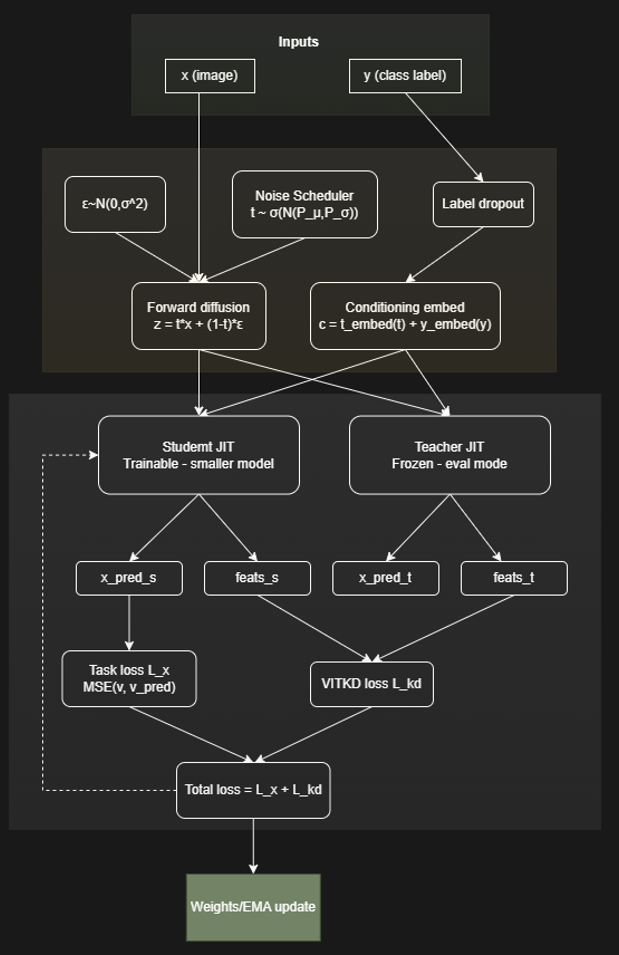
\includegraphics[width=0.92\linewidth]{figures/formula/training-loop.png}
    \caption{Overview of the proposed knowledge distillation framework. The teacher JiT model (larger variant) is frozen and processes the same noisy input as the student (smaller variant) at every training step. Three distillation signals are derived from the teacher: (i) intermediate feature maps from shallow and deep transformer blocks, used by the ViTKD loss; (ii) post-softmax self-attention weight matrices from the final $K$ blocks, used by the attention KD loss; and (iii) a structured subset of pretrained weights, used to initialise the student prior to training. The student is additionally supervised by the standard flow-matching denoising loss $\mathcal{L}_{\text{flow}}$. At inference time, only the student is used.}
    \label{fig:framework_overview}
\end{figure}


% ============================================================
\section{Feature Map Distillation via ViTKD}
\label{sec:vitkd}
% ============================================================

\subsection{Motivation: Feature Distillation for Vision Transformers}
\label{subsec:vitkd_motivation}

Feature-based knowledge distillation has a long history in the context of convolutional neural networks (CNNs), tracing back to the seminal FitNets framework \cite{romero2015fitnets}, which proposed to match intermediate feature maps between teacher and student networks via a regression objective. Subsequent works refined this idea through attention-based feature transfer \cite{zagoruyko2017paying}, relational feature distillation \cite{park2019relational}, and various forms of channel-wise or spatial normalisation \cite{heo2019comprehensive}. These methods, however, were designed with the specific inductive biases of CNNs in mind: hierarchical spatial resolution, local receptive fields, and feature maps with explicit channel-height-width structure. When applied naïvely to Vision Transformers \cite{dosovitskiy2020vit}, they tend to be ineffective or even detrimental, owing to the fundamental architectural differences: ViTs operate on a flat sequence of patch tokens with a fixed spatial resolution throughout, no pooling hierarchy, and feature representations that encode information in a distributed, non-local manner across the sequence dimension.

Responding to this gap, \cite{yang2022vitkd} conducted a systematic empirical study of feature distillation strategies tailored specifically to ViTs. Through a series of controlled ablations, they derived three practical guidelines that deviate substantially from CNN-era conventions. First, \emph{shallow transformer layers} are best distilled via direct mimicking: aligning the student's early hidden states to the teacher's counterparts through a simple learned linear projection, supervised by a mean squared error objective. In contrast to CNN practices, where shallow feature distillation is often less informative than deep feature distillation, shallow ViT layers attend to low-level structural patterns and positional relationships that are foundational to the subsequent processing of the sequence; transferring them directly proves highly beneficial. Second, \emph{deep transformer layers} are best distilled via a generative reconstruction objective: a fraction of the student's final-layer tokens are masked and replaced with a learned mask token, and a lightweight convolutional projector is trained to reconstruct the teacher's corresponding deep features at the masked positions. This forces the student to capture the global context and high-level semantic structure encoded in the teacher's final hidden states, rather than merely performing local point-wise regression. Third, a simple linear projection is sufficient for dimension alignment between teacher and student embedding spaces; elaborate multi-layer projection heads introduce unnecessary optimisation difficulty and degrade distillation performance. On ImageNet-1K image classification with DeiT architectures, this framework, termed ViTKD, yields consistent and significant improvements across multiple student sizes \cite{yang2022vitkd}.

The applicability of ViTKD to diffusion model distillation is non-trivial, but its core principles are well-motivated in this context. In JiT, the transformer blocks process patch token sequences derived directly from noisy pixel-space images, and the resulting feature representations are conditioned on both the class label $y$ and the continuous noise level $t$. Early blocks encode coarse low-level denoising patterns, positional structure, and texture statistics, while the final block aggregates global contextual information that determines the model's final velocity prediction $v_\theta(\mathbf{z}, t, y)$. Supervising the student's intermediate representations to match those of a larger teacher thus exerts pressure for the student to develop more accurate and better-calibrated internal models of the denoising process, which translates directly into higher generative quality.

\subsection{Adapting ViTKD to the Diffusion Setting}
\label{subsec:vitkd_adaptation}

Although the architectural backbone is shared — both the original ViTKD and our setting involve a pair of Vision Transformers of differing capacities — several non-trivial adaptations are required to apply ViTKD effectively to a conditional diffusion model. The central challenge is that, unlike a classification network whose internal representations are conditioned only on the input image, the hidden states of a diffusion model are explicitly conditioned on the noise level $t \in [0, 1]$. In JiT, this conditioning is implemented via adaptive layer normalisation (adaLN) \cite{peebles2023scalable}, in which each transformer block computes per-block shift and scale vectors from a conditioning signal $\mathbf{c} \in \mathbb{R}^{D}$ that fuses the timestep embedding and the class embedding. As a result, the statistical properties of the intermediate hidden states — their scale, orientation in embedding space, and distributional shape — vary substantially across the denoising trajectory. A plain linear alignment layer $\phi: \mathbb{R}^{D_S} \to \mathbb{R}^{D_T}$, as prescribed in the original ViTKD, is a static affine map that cannot account for this trajectory-dependent variation and may therefore produce a poorly calibrated distillation objective at certain noise levels.

To address this, we introduce a \textbf{timestep-conditioned alignment layer}, which we term \texttt{AdaLNAlign}. Rather than applying a bare linear projection, the aligned feature is modulated by an adaLN operation conditioned on the student's conditioning vector $\mathbf{c}$:
%
\begin{equation}
    \phi_i^{\text{AdaLN}}(\mathbf{F}_i^S, \mathbf{c}) = \left(1 + \boldsymbol{\gamma}_i(\mathbf{c})\right) \odot \mathbf{W}_i \mathbf{F}_i^S + \boldsymbol{\delta}_i(\mathbf{c}),
    \label{eq:adaln_align}
\end{equation}
%
where $\mathbf{F}_i^S \in \mathbb{R}^{B \times N \times D_S}$ denotes the student's feature tensor at shallow layer $i$, $\mathbf{W}_i \in \mathbb{R}^{D_T \times D_S}$ is a learnable linear projection, and the per-token shift and scale vectors $\boldsymbol{\delta}_i(\mathbf{c}), \boldsymbol{\gamma}_i(\mathbf{c}) \in \mathbb{R}^{B \times N \times D_T}$ are produced by a two-layer MLP applied to $\mathbf{c}$ and broadcast over the token dimension. The MLP's output layer is initialised to zero, ensuring that at the start of training the alignment degenerates to a plain linear projection, and the modulation is learned progressively. This design allows the alignment layer to dynamically rescale and shift the student's features according to the current noise level before computing the mimicking loss, thereby normalising out trajectory-induced distributional variation.

A second adaptation concerns the weighting of individual training samples in the distillation loss. At extreme noise levels, particularly for $t$ close to zero or one, the signal-to-noise ratio (SNR) of the noisy input $\mathbf{z} = t\mathbf{x} + (1-t)\mathbf{e}$ is either very high (nearly clean) or very low (nearly pure noise), and the gradients produced by the distillation loss at these regimes tend to be either trivially small or dominated by noise artefacts. To mitigate this, we adopt \textbf{Min-SNR-$\gamma$ loss weighting} \cite{hang2023efficient}, which assigns per-sample weights $w(t)$ based on the effective SNR of the training sample:
%
\begin{equation}
    \mathrm{SNR}(t) = \left( \frac{t}{1 - t} \right)^2, \qquad w(t) = \frac{\min\!\left(\mathrm{SNR}(t),\, \gamma\right)}{\gamma},
    \label{eq:snr_weight}
\end{equation}
%
where $\gamma > 0$ is a clipping hyperparameter that prevents samples with very high SNR from dominating the loss. When $\gamma = 0$, the weighting is disabled and all samples are treated uniformly. This weighting is applied to both the mimicking and generation components of the ViTKD loss.


\subsection{Shallow-Layer Mimicking Loss}
\label{subsec:vitkd_mimic}

The mimicking component of ViTKD operates on the output hidden states of the first two transformer blocks of both teacher and student. Let $\mathbf{F}_i^S \in \mathbb{R}^{B \times N \times D_S}$ and $\mathbf{F}_i^T \in \mathbb{R}^{B \times N \times D_T}$ denote the post-block feature tensors of the student and teacher at shallow layer $i \in \{0, 1\}$, respectively, where $B$ is the batch size, $N$ is the number of patch tokens, and $D_S$, $D_T$ are the respective embedding dimensions. When $D_S \neq D_T$, dimension alignment is required before computing the loss. Depending on whether timestep conditioning is enabled, the alignment is performed by either the \texttt{AdaLNAlign} module introduced in Equation~\eqref{eq:adaln_align} or a plain learned linear projection $\mathbf{W}_i \in \mathbb{R}^{D_T \times D_S}$. In both cases, the aligned student feature is denoted $\hat{\mathbf{F}}_i^S \in \mathbb{R}^{B \times N \times D_T}$.

The mimicking loss is then computed as a mean squared error between aligned student features and the corresponding teacher features, summed over the two shallow layers and normalised by batch size:
%
\begin{equation}
    \mathcal{L}_{\text{mimic}} = \frac{\alpha}{B} \sum_{i=0}^{1} \sum_{b=1}^{B} w(t_b) \cdot \left\| \hat{\mathbf{F}}_{i,b}^S - \mathbf{F}_{i,b}^T \right\|_F^2,
    \label{eq:loss_mimic}
\end{equation}
%
where $\alpha$ is a scalar loss weight, $w(t_b)$ is the Min-SNR-$\gamma$ weight for sample $b$ (equal to 1 when weighting is disabled), and $\|\cdot\|_F^2$ denotes the squared Frobenius norm over the token and channel dimensions. The alignment layers $\{\mathbf{W}_i\}_{i=0}^{1}$ are the only learnable parameters introduced by this component; they are trained jointly with the student network via backpropagation. The teacher features $\mathbf{F}_i^T$ are computed under \texttt{torch.no\_grad()} and treated as fixed targets.

In the JiT architecture, the first two transformer blocks operate on the patch embedding before the deeper adaLN-modulated blocks begin to integrate strong class and noise-level conditioning. Their outputs therefore reflect a relatively stable, low-level decomposition of the input, making them suitable targets for direct regression. The mimicking loss exerts a force that aligns the student's early computational pathway to the teacher's, promoting the development of analogous low-level feature detectors.


\subsection{Deep-Layer Generation Loss}
\label{subsec:vitkd_gen}

The generation component of ViTKD targets the output hidden states of the final transformer block of both teacher and student. Let $\mathbf{H}^S \in \mathbb{R}^{B \times N \times D_S}$ and $\mathbf{H}^T \in \mathbb{R}^{B \times N \times D_T}$ denote these deep features. The rationale for treating shallow and deep layers differently is that the final-block representations in a trained ViT encode high-level, globally integrated semantic information that is difficult to transfer via direct regression: a student with insufficient capacity may simply overfit to matching the teacher's final features locally without developing the underlying distributed processing structure required to produce them. The generation objective sidesteps this issue by introducing a reconstruction task under partial information, compelling the student to leverage global context rather than performing local point-wise imitation.

The procedure operates as follows. The student's deep features $\mathbf{H}^S$ are first linearly projected to the teacher's dimension: $\tilde{\mathbf{H}}^S = \mathbf{W}_{\text{deep}} \mathbf{H}^S$, where $\mathbf{W}_{\text{deep}} \in \mathbb{R}^{D_T \times D_S}$. A random binary mask $\mathbf{m} \in \{0, 1\}^{B \times N}$ is then sampled per batch, with each token independently masked with probability $\lambda \in (0, 1)$. Masked token positions in $\tilde{\mathbf{H}}^S$ are replaced with a shared learnable mask token $\boldsymbol{\mu} \in \mathbb{R}^{1 \times 1 \times D_T}$, broadcast over the batch and masked positions. The resulting partially-masked sequence is reshaped from its flat token representation $\mathbb{R}^{B \times N \times D_T}$ into a spatial grid $\mathbb{R}^{B \times D_T \times \sqrt{N} \times \sqrt{N}}$, passed through a lightweight convolutional projector consisting of two $3 \times 3$ convolutions with a ReLU nonlinearity, and then reshaped back to the token format. The generation loss is computed only on the masked positions, measuring how well the projector can reconstruct the teacher's deep features at those locations using the spatial context provided by the surrounding unmasked tokens:
%
\begin{equation}
    \mathcal{L}_{\text{gen}} = \frac{\beta}{B \lambda} \sum_{b=1}^{B} w(t_b) \cdot \left\| \left( \hat{\mathbf{H}}_b^S - \mathbf{H}_b^T \right) \odot \mathbf{m}_b \right\|_F^2,
    \label{eq:loss_gen}
\end{equation}
%
where $\hat{\mathbf{H}}_b^S$ denotes the projector output for sample $b$, $\mathbf{m}_b \in \{0,1\}^{N \times 1}$ is the per-sample mask broadcast over the channel dimension, $\beta$ is a scalar loss weight, and the $\lambda$ factor in the denominator normalises for the varying number of masked tokens. The mask is sampled uniformly at random without replacement using a noise-based shuffling procedure \cite{he2022masked}. In practice, $\lambda = 0.5$ is used as the default masking ratio, meaning that half of the student's deep tokens are masked per step.

The convolutional projector is the critical architectural element distinguishing the generation component from a second mimicking term: by requiring the model to spatially interpolate across masked positions using a $3 \times 3$ receptive field, it forces the student's projected features to encode local spatial coherence consistent with the teacher's global deep representation. This is particularly meaningful in the diffusion context, where the final-block features must ultimately support a spatially consistent velocity prediction across the entire image.

An ablation mode \texttt{mimic\_only} is provided, in which the generation loss is omitted entirely and only $\mathcal{L}_{\text{mimic}}$ is applied. This configuration is investigated experimentally in Chapter~\ref{chap:experiments} to isolate the contribution of each component.


\subsection{Total ViTKD Loss}
\label{subsec:vitkd_total}

The overall ViTKD distillation loss is the sum of the shallow-layer mimicking loss and the deep-layer generation loss:
%
\begin{equation}
    \mathcal{L}_{\text{ViTKD}} = \mathcal{L}_{\text{mimic}} + \mathcal{L}_{\text{gen}},
    \label{eq:loss_vitkd}
\end{equation}
%
where $\mathcal{L}_{\text{mimic}}$ and $\mathcal{L}_{\text{gen}}$ are as defined in Equations~\eqref{eq:loss_mimic} and~\eqref{eq:loss_gen}, respectively. The two terms are independently scaled by $\alpha$ and $\beta$, with default values $\alpha = 3 \times 10^{-5}$ and $\beta = 3 \times 10^{-6}$, reflecting the fact that the generation loss is applied to a smaller subset of tokens and its gradient norm would otherwise dominate at higher values. During training, $\mathcal{L}_{\text{ViTKD}}$ is added to the primary flow-matching denoising loss of the student, described in Section~\ref{sec:unified_objective}. The learnable parameters introduced by ViTKD — the alignment layers $\{\mathbf{W}_i\}$, the deep alignment layer $\mathbf{W}_{\text{deep}}$, the mask token $\boldsymbol{\mu}$, and the convolutional projector — are trained jointly with the student network. A summary of all ViTKD hyperparameters is provided in Table~\ref{tab:vitkd_hyperparams}.

\begin{table}[ht]
    \centering
    \caption{Summary of ViTKD hyperparameters, their default values, the ranges explored during ablation, and their functional role in the distillation objective. Full ablation results are reported in Chapter~\ref{chap:experiments}.}
    \label{tab:vitkd_hyperparams}
    \begin{tabular}{lccl}
        \toprule
        \textbf{Hyperparameter} & \textbf{Symbol} & \textbf{Default} & \textbf{Role} \\
        \midrule
        Mimicking loss weight   & $\alpha$             & $3 \times 10^{-5}$ & Scales $\mathcal{L}_{\text{mimic}}$ \\
        Generation loss weight  & $\beta$              & $3 \times 10^{-6}$ & Scales $\mathcal{L}_{\text{gen}}$ \\
        Masking ratio           & $\lambda$            & $0.5$              & Fraction of deep tokens masked \\
        Min-SNR clipping        & $\gamma$             & $0.0$ (disabled)   & Controls SNR-based loss weighting \\
        Time conditioning       & ---                  & disabled           & Enables \texttt{AdaLNAlign} vs.\ plain linear \\
        Mimicking only          & ---                  & disabled           & Ablates generation loss \\
        \bottomrule
    \end{tabular}
\end{table}

\begin{figure}[ht]
    \centering
    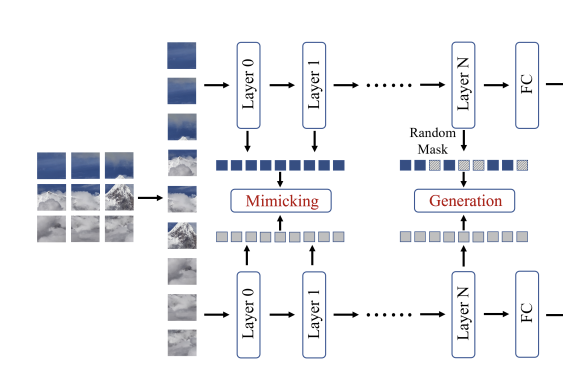
\includegraphics[width=\linewidth]{figures/formula/VITKD.png}
    \caption{Detailed schematic of the ViTKD distillation pipeline applied to the JiT teacher--student pair. \textbf{Top path (mimicking):} hidden-state tensors $\mathbf{F}_i^T$ and $\mathbf{F}_i^S$ from the first two transformer blocks of teacher and student, respectively, are aligned via learned projections $\phi_i$ (plain linear or \texttt{AdaLNAlign}) and compared under an MSE loss $\mathcal{L}_{\text{mimic}}$. \textbf{Bottom path (generation):} the student's final-block features $\mathbf{H}^S$ are linearly projected to $D_T$ dimensions, a random subset of tokens is masked (shown in grey), and a convolutional projector reconstructs the masked positions from spatial context; the reconstruction error against the teacher's final features $\mathbf{H}^T$ defines $\mathcal{L}_{\text{gen}}$. The conditioning vector $\mathbf{c}$ (encoding timestep and class) feeds the \texttt{AdaLNAlign} modulation when timestep conditioning is enabled. All teacher computations are performed without gradient tracking. Dimension annotations: $D_S$ and $D_T$ denote student and teacher embedding dimensions, respectively; $N$ denotes the number of patch tokens.}
    \label{fig:vitkd_pipeline}
\end{figure}

% ============================================================
\section{Attention Map Distillation}
\label{sec:attn_kd}
% ============================================================

A central finding of the recent work by \citet{li2024attentiontransfer} (NeurIPS 2024) challenges the conventional understanding of what pre-training accomplishes in Vision Transformers. The authors demonstrate that the specific feature representations learned during pre-training are not essential to recover its downstream benefits; rather, it is the \emph{attention patterns} — the learned distributions over which tokens attend to which — that constitute the primary carrier of transferable knowledge. They formalise this observation through a method called attention transfer, in which only the post-softmax attention weight matrices of a pretrained teacher ViT are used to supervise a student, while the student is free to develop its own feature representations from scratch. In the attention distillation variant of their framework, the student computes its own attention maps and is trained with an auxiliary cross-entropy loss that encourages those maps to match the teacher's. Despite its simplicity, this approach recovers most of the accuracy gap between training from scratch and full weight fine-tuning on ImageNet-1K classification.

This finding is particularly well-motivated in the pixel-space diffusion setting of JiT. At each denoising timestep $t$, the multi-head self-attention maps of a JiT block directly encode spatial relationships between image patch tokens: which patches attend to which others, reflecting spatial proximity, texture coherence, semantic grouping, and structural layout at the pixel level. Because JiT operates on raw pixel patches rather than abstract latent codes, these attention distributions carry a direct and interpretable correspondence to image content. A teacher model that has been trained to convergence will have developed refined attention routing — grouping semantically related patches, suppressing noisy or uninformative tokens, and resolving long-range spatial dependencies — that a smaller student model has insufficient capacity to discover independently within the same training budget. Supervising the student's attention distributions to approximate those of the teacher therefore transfers a form of relational inductive bias that cannot be conveyed by the output-level flow-matching loss alone.

\subsection*{Attention Map Extraction and Preprocessing}

Attention maps are extracted from the last $K$ transformer blocks of both teacher and student, where $K$ is a hyperparameter (\texttt{num\_attn\_layers}, default $K = 2$). Within each selected block, each of the $H$ attention heads produces a matrix $\mathbf{A} \in \mathbb{R}^{N_{\text{total}} \times N_{\text{total}}}$, where $N_{\text{total}}$ includes both the image patch tokens $N$ and the in-context conditioning tokens appended by JiT's in-context conditioning mechanism. Before the distillation loss is computed, two preprocessing steps are applied. First, the in-context conditioning tokens are stripped, reducing each attention matrix to $\mathbb{R}^{N \times N}$, so that the supervision signal concerns only the spatial routing among image patch tokens and is not confounded by the conditioning tokens. Second, the $H$ per-head maps are averaged across the head dimension to produce a single head-averaged map $\bar{\mathbf{A}} \in \mathbb{R}^{N \times N}$ per block; rows are then renormalised to sum to one, ensuring each row remains a valid probability distribution over the $N$ key positions. This head-averaging strategy is adopted for tractability and consistency: the teacher and student may in general have different numbers of attention heads ($H_T \neq H_S$), and aligning individual heads across architectures introduces an arbitrary correspondence problem. Head-averaging sidesteps this issue cleanly, producing a common spatial routing distribution that is architecture-agnostic.

\subsection*{Distillation Objective: KL Divergence}

Let $\bar{\mathbf{A}}_S^{(\ell)} \in \mathbb{R}^{B \times N \times N}$ and $\bar{\mathbf{A}}_T^{(\ell)} \in \mathbb{R}^{B \times N \times N}$ denote the preprocessed, head-averaged attention maps of the student and teacher at selected layer $\ell \in \{1, \ldots, K\}$, respectively. The attention distillation loss penalises distributional discrepancy between corresponding student and teacher attention maps. Whereas the original attention transfer paper of \cite{li2024attentiontransfer} employs cross-entropy $H(\bar{\mathbf{A}}_T^{(\ell)}, \bar{\mathbf{A}}_S^{(\ell)})$ as the distillation objective, we adopt the Kullback-Leibler (KL) divergence as the primary loss function. This choice is motivated by the fact that the rows of $\bar{\mathbf{A}}$ are proper probability distributions over the $N$ token positions; KL divergence is the canonical information-theoretic measure of how much one distribution diverges from another, and unlike cross-entropy it is invariant to the entropy of the target distribution, making the loss magnitude more interpretable and stable across different noise levels $t$ where the teacher's attention entropy may vary significantly.

For each query token position $n \in \{1, \ldots, N\}$ and each selected layer $\ell$, the KL divergence from the student's distribution to the teacher's is:
%
\begin{equation}
    D_{\mathrm{KL}}\!\left(\bar{\mathbf{A}}_{T,n}^{(\ell)} \,\big\|\, \bar{\mathbf{A}}_{S,n}^{(\ell)}\right)
    = \sum_{n'=1}^{N} \bar{A}_{T,n,n'}^{(\ell)} \log \frac{\bar{A}_{T,n,n'}^{(\ell)}}{\bar{A}_{S,n,n'}^{(\ell)}},
    \label{eq:kl_per_query}
\end{equation}
%
where $\bar{A}_{T,n,n'}^{(\ell)}$ denotes the $(n, n')$ entry of the teacher's head-averaged attention map at layer $\ell$. The full attention distillation loss aggregates over all query tokens, batch samples, and selected layers:
%
\begin{equation}
    \mathcal{L}_{\text{attn}} = \frac{\gamma}{K} \sum_{\ell=1}^{K} \frac{1}{B'} \sum_{b=1}^{B'} \frac{1}{N} \sum_{n=1}^{N} D_{\mathrm{KL}}\!\left(\bar{\mathbf{A}}_{T,b,n}^{(\ell)} \,\big\|\, \bar{\mathbf{A}}_{S,b,n}^{(\ell)}\right),
    \label{eq:loss_attn}
\end{equation}
%
where $\gamma$ is a scalar loss weight (\texttt{gamma\_attn}, default $\gamma = 10^{-4}$), $B' \leq B$ is the number of samples in the batch that pass the timestep gate (described below), and the division by $K$ normalises the loss magnitude to be independent of the number of supervised layers. A numerical stability offset $\varepsilon = 10^{-8}$ is added to all attention weights before computing the logarithm, followed by a renormalisation pass to ensure strict distributional validity. We additionally investigate a \textbf{symmetric} variant of the loss, defined as $\frac{1}{2}\left[D_{\mathrm{KL}}(\bar{\mathbf{A}}_T \| \bar{\mathbf{A}}_S) + D_{\mathrm{KL}}(\bar{\mathbf{A}}_S \| \bar{\mathbf{A}}_T)\right]$, which penalises divergence in both directions and may be preferable when the student and teacher attention distributions overlap substantially. The asymmetric variant (default) enforces a one-directional pressure pushing the student toward the teacher without penalising the student for distributing probability mass differently in regions the teacher ignores.

\subsection*{Timestep Gating}

A critical consideration specific to the diffusion setting is that at very low noise levels — concretely, for $t \leq t_{\min}$ (default $t_{\min} = 0.1$) — the noisy input $\mathbf{z} = t\mathbf{x} + (1-t)\mathbf{e}$ is dominated by Gaussian noise and carries negligible image content. In this regime, the attention maps of both teacher and student tend toward near-uniform distributions, as no meaningful spatial structure is recoverable from the near-pure-noise input. Supervising the student to match the teacher's near-uniform attention at these timesteps would inject gradient noise rather than useful signal, potentially destabilising training. Accordingly, any sample $b$ in the batch for which $t_b \leq t_{\min}$ is excluded from $\mathcal{L}_{\text{attn}}$: the gated batch size $B'$ in Equation~\eqref{eq:loss_attn} counts only those samples for which $t_b > t_{\min}$. If all samples in a batch fall below this threshold, the attention loss evaluates to zero for that step. The full set of hyperparameters governing the attention distillation loss is summarised in Table~\ref{tab:attn_hyperparams}.

\begin{table}[ht]
    \centering
    \caption{Hyperparameters of the attention map distillation loss. Default values reflect those used in the primary experimental configuration; ablation over selected hyperparameters is reported in Chapter~\ref{chap:experiments}.}
    \label{tab:attn_hyperparams}
    \begin{tabular}{lccl}
        \toprule
        \textbf{Hyperparameter} & \textbf{Symbol} & \textbf{Default} & \textbf{Role} \\
        \midrule
        Attention loss weight    & $\gamma$       & $10^{-4}$         & Overall scale of $\mathcal{L}_{\text{attn}}$ \\
        Number of supervised layers & $K$         & $2$               & Last $K$ blocks used for supervision \\
        Timestep gate threshold  & $t_{\min}$    & $0.1$             & Excludes near-noise samples \\
        Numerical stability      & $\varepsilon$ & $10^{-8}$         & Added before log to prevent $\log(0)$ \\
        Symmetric KL             & ---           & enabled           & Uses $\frac{1}{2}(\mathrm{KL}_{T\to S} + \mathrm{KL}_{S\to T})$ \\
        \bottomrule
    \end{tabular}
\end{table}

\begin{figure}[ht]
    \centering
    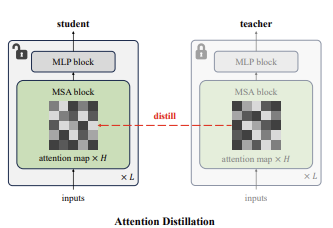
\includegraphics[width=\linewidth]{figures/formula/attn-d.png}
    \caption{Illustration of the attention map distillation procedure. From each of the last $K$ transformer blocks, the $H$ per-head attention matrices are extracted from both teacher (frozen) and student (trainable), averaged across heads, and stripped of in-context conditioning tokens to yield spatial routing distributions $\bar{\mathbf{A}}_T^{(\ell)}, \bar{\mathbf{A}}_S^{(\ell)} \in \mathbb{R}^{N \times N}$. Samples with $t \leq t_{\min}$ are excluded (greyed out). KL divergence is computed between the resulting distributions and aggregated across layers and tokens to form $\mathcal{L}_{\text{attn}}$. No learnable parameters are introduced by this component; the student's attention maps are computed by its own multi-head self-attention mechanism.}
    \label{fig:attn_kd_pipeline}
\end{figure}

The attention distillation component introduces no learnable parameters: the student's attention maps are produced by its own query--key dot-product mechanism, and no projection or alignment layer is required because both teacher and student produce head-averaged maps of the same spatial dimension $N \times N$, regardless of their respective embedding dimensions or head counts. This makes the attention loss computationally inexpensive relative to the ViTKD feature distillation, as it requires only the collection of attention weight matrices during the student and teacher forward passes — operations that are already performed internally and need only be returned rather than discarded.


% ============================================================
\section{Weight Selection as Complementary Initialisation}
\label{sec:weight_selection}
% ============================================================

The two distillation methods described in Sections~\ref{sec:vitkd} and~\ref{sec:attn_kd} are \emph{online} training objectives: they are evaluated and differentiated at every gradient step throughout the entire training run. Weight selection \cite{xu2024initializing}, by contrast, is an \emph{offline} initialisation strategy that is applied once, before any gradient update, and whose effect is therefore mediated entirely through the quality of the student's starting point on the loss landscape. It is nonetheless a meaningful component of the framework, as the starting point from which distillation training begins can substantially influence both the convergence speed and the quality of the eventual solution.

\subsection*{Method}

\cite{xu2024initializing} (ICLR 2024, Spotlight) introduce weight selection as a general technique for initialising a smaller model by extracting a structured subset of weights from a larger, pretrained counterpart. The key observation motivating the method is that, in the large-model era, pretrained weights encode learned representations, inductive biases, and optimised parameter configurations that took substantial compute to acquire. Discarding this information entirely in favour of random initialisation — as is standard practice when training a smaller model from scratch — is unnecessarily wasteful. Weight selection proposes instead to \emph{inherit} a portion of the teacher's learned knowledge directly through the initialisation of the student's parameters, at zero additional training cost.

The initialisation procedure operates parameter-tensor by parameter-tensor. For each learnable parameter key $k$ present in both teacher and student state dictionaries, the following cases are handled. If the teacher and student tensors at key $k$ have identical shapes, the teacher tensor is copied directly into the student. If the teacher tensor is strictly larger than the student tensor in one or more dimensions — which is the generic case when the student has fewer hidden units or fewer layers — a \emph{uniform element selection} is applied: for each dimension $d$ in which the shapes differ, a set of $s_d$ indices is drawn at uniform spacing from the teacher's $t_d$ entries, where $s_d$ and $t_d$ are the student and teacher sizes along dimension $d$, respectively. When $t_d$ is divisible by $s_d$, a regular stride of $t_d / s_d$ is used; otherwise, indices are computed via evenly-spaced linspace rounding. This selection is applied sequentially across all differing dimensions, yielding a student-shaped sub-tensor drawn from the teacher. Parameters for which the teacher tensor is smaller than the student tensor in any dimension, or whose key is absent from the teacher's state dictionary, are left at their default random initialisation.

\subsection*{Application to JiT and Handling of Architectural Mismatches}

Applying weight selection to the JiT model family requires careful handling of several architecture-specific considerations. The primary cases encountered in our experimental pairs are summarised as follows.

\paragraph{Hidden dimension reduction.} In the CIFAR-10 setting, the teacher is JiT-S/2 with hidden dimension $D_T = 512$ and the student is JiT-T/2 with $D_S = 384$. All weight matrices of the form $\mathbf{W} \in \mathbb{R}^{D_T \times D_T}$ — including query, key, value, and projection weight matrices in every attention block, as well as FFN weight matrices — are reduced to $\mathbb{R}^{D_S \times D_S}$ by uniform selection along both dimensions. In the ImageNet setting, the teacher is JiT-B/16 with $D_T = 768$ and the student is JiT-S/16 with $D_S = 384$; the same procedure applies.

\paragraph{Depth reduction.} In the CIFAR-10 pair, the teacher has 10 transformer blocks and the student has 6. Since the student has fewer layers, the selected layers must be chosen from the teacher's depth. In our implementation, the student's layers are matched to the teacher's by a uniform stride across the teacher's block indices, preserving early and late layers which encode respectively the low-level denoising patterns and the high-level velocity prediction structure.

\paragraph{Non-learnable and regenerated parameters.} Positional embedding buffers (\texttt{pos\_embed}), rotary embedding frequency tensors (\texttt{freqs\_cos}, \texttt{freqs\_sin}), and similar deterministic buffers are excluded from weight selection and recomputed from the student's own configuration. These quantities depend on the model's spatial resolution and sequence length and cannot be meaningfully inherited from the teacher.

\paragraph{Class embedding remapping.} When the teacher was trained on a dataset with a different number of classes than the student's target (e.g., a teacher pretrained on ImageNet-1K being adapted to CIFAR-10), the class embedding table $\mathbf{E}_y \in \mathbb{R}^{(C+1) \times D}$ — where $C$ is the number of classes and the extra row corresponds to the unconditional null class — has incompatible first dimensions. In this case, the class embeddings are excluded from weight selection and re-initialised randomly in the student. This is an expected and handled edge case in our codebase.

\subsection*{Role Within the Framework}

Weight selection is complementary to the ViTKD and attention distillation losses in a precise sense: it does not introduce any additional loss term, does not modify the training loop, and does not impose any computational overhead during training. Its benefit is expressed entirely through the starting configuration of the student's parameters. A student initialised via weight selection begins its training in a region of parameter space that is structurally similar to a converged teacher — its attention heads already encode meaningful queries and keys, its MLP weights already perform useful feature transformations, and its adaLN modulation layers are already calibrated to reasonable scale and shift ranges. This informed starting point means that the ViTKD and attention distillation losses, which provide supervision from the teacher's internal representations throughout training, operate on a student that is already in approximate alignment with the teacher from step zero, rather than having to first correct the large initial mismatch that would arise from random initialisation. Empirically, this is expected to translate into faster convergence and potentially higher final performance, as the distillation losses can focus on refining rather than bootstrapping the student's representations. The combination of weight selection initialisation with online distillation training is accordingly the recommended default configuration of the proposed framework.

\begin{figure}[ht]
    \centering
    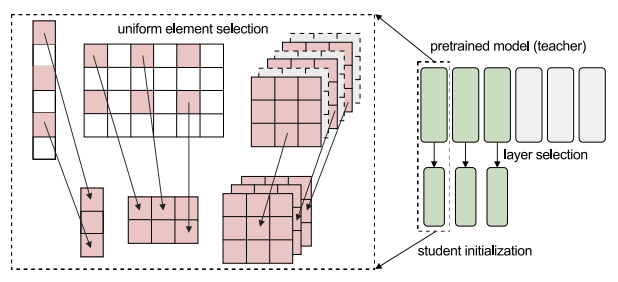
\includegraphics[width=0.85\linewidth]{figures/formula/weight-selection.png}
    \caption{Illustration of the weight selection initialisation procedure for the JiT-S/2 $\to$ JiT-T/2 pair ($D_T = 512$, $D_S = 384$, teacher depth 10, student depth 6). \textbf{Left:} for each weight matrix, a structured subset of rows and columns is selected at uniform spacing from the teacher tensor (shown in orange), yielding a student-sized initialisation (shown in blue). \textbf{Right:} layer correspondence for the depth reduction case; the student's 6 blocks are matched to 6 of the teacher's 10 blocks at uniform stride, preserving both early and late layers.}
    \label{fig:weight_selection}
\end{figure}


% ============================================================
\section{Unified Training Objective}
\label{sec:unified_objective}
% ============================================================

The three components described in the preceding sections are integrated into a single training procedure. Weight selection provides a one-time initialisation of the student's parameters from the teacher's pretrained weights before training commences. During each subsequent training step, the student is optimised under a combined loss that aggregates the base denoising objective with the two distillation losses:
%
\begin{equation}
    \mathcal{L}_{\text{total}} = \mathcal{L}_{\text{flow}} + \mathcal{L}_{\text{ViTKD}} + \mathcal{L}_{\text{attn}},
    \label{eq:loss_total}
\end{equation}
%
where each term serves a distinct supervisory role. The flow-matching denoising loss $\mathcal{L}_{\text{flow}}$ ensures that the student remains a well-formed generative model, trained to predict the velocity field of the probability flow ODE for the data distribution. For a batch of clean images $\mathbf{x}$ and class labels $y$, with noise $\mathbf{e} \sim \mathcal{N}(\mathbf{0}, \sigma^2 \mathbf{I})$ and timestep $t$ sampled from a log-normal distribution mapped through the sigmoid function, the noisy input is $\mathbf{z} = t\mathbf{x} + (1-t)\mathbf{e}$ and the target velocity is $\mathbf{v} = (\mathbf{x} - \mathbf{z}) / (1 - t)$. The denoising loss is:
%
\begin{equation}
    \mathcal{L}_{\text{flow}} = \mathbb{E}_{t, \mathbf{x}, \mathbf{e}, y}\!\left[ \left\| \mathbf{v}_\theta(\mathbf{z}, t, y) - \mathbf{v} \right\|_2^2 \right],
    \label{eq:loss_flow}
\end{equation}
%
where $\mathbf{v}_\theta$ denotes the student's velocity prediction. The ViTKD loss $\mathcal{L}_{\text{ViTKD}} = \mathcal{L}_{\text{mimic}} + \mathcal{L}_{\text{gen}}$ (Equation~\eqref{eq:loss_vitkd}) transfers intermediate feature map knowledge from the teacher's shallow and deep transformer blocks. The attention distillation loss $\mathcal{L}_{\text{attn}}$ (Equation~\eqref{eq:loss_attn}) transfers the teacher's learned spatial routing patterns. The relative magnitudes of the three loss components are governed by the hyperparameters $\alpha$, $\beta$, and $\gamma$; in practice, $\mathcal{L}_{\text{flow}}$ is of order one, while $\mathcal{L}_{\text{ViTKD}}$ and $\mathcal{L}_{\text{attn}}$ are scaled to be approximately one to two orders of magnitude smaller, ensuring that the distillation signal acts as a regulariser on the student's internal representations without displacing the primary generative objective.

The teacher's weights are held frozen for the entirety of training. Concretely, no gradients are propagated through the teacher's parameters at any point; all teacher forward passes are executed under \texttt{torch.no\_grad()}. The only parameters updated by backpropagation are those of the student network and the ViTKD alignment layers ($\{\mathbf{W}_i\}$, $\mathbf{W}_{\text{deep}}$, $\boldsymbol{\mu}$, and the convolutional projector weights). The attention distillation component introduces no additional learnable parameters. Following each gradient update, an exponential moving average (EMA) of the student's parameters is maintained — independently of the teacher — and used for all generation and evaluation passes. Algorithm~\ref{alg:distill_training} provides a concise summary of one complete training step.

\begin{algorithm}[ht]
\caption{One Training Step of the Distillation Framework}
\label{alg:distill_training}
\begin{algorithmic}[1]
    \Require Clean images $\mathbf{x}$, class labels $y$; frozen teacher $f_T$; student $f_S$ (trainable); ViTKD loss module $\mathcal{L}_{\text{ViTKD}}$; attention KD loss module $\mathcal{L}_{\text{attn}}$
    \State Sample $t \sim \sigma({\mathcal{N}(\mu_P, \sigma_P^2)})$, $\mathbf{e} \sim \mathcal{N}(\mathbf{0}, \sigma_{\text{noise}}^2\mathbf{I})$
    \State $\mathbf{z} \leftarrow t\mathbf{x} + (1-t)\mathbf{e}$ \Comment{Construct noisy image}
    \State $\mathbf{v} \leftarrow (\mathbf{x} - \mathbf{z}) / (1-t)$ \Comment{Target velocity}
    \State $\hat{\mathbf{v}}_S,\, \mathbf{F}_S,\, \mathbf{A}_S \leftarrow f_S(\mathbf{z}, t, y)$ \Comment{Student forward pass; collect features and attention maps}
    \State $\mathcal{L}_{\text{flow}} \leftarrow \|\hat{\mathbf{v}}_S - \mathbf{v}\|_2^2$
    \State \textbf{with} \texttt{no\_grad():}
    \State \quad $\mathbf{F}_T,\, \mathbf{A}_T \leftarrow f_T(\mathbf{z}, t, y)$ \Comment{Teacher forward pass; no gradient}
    \State $\mathcal{L}_{\text{ViTKD}} \leftarrow \mathcal{L}_{\text{mimic}}(\mathbf{F}_S^{\text{low}}, \mathbf{F}_T^{\text{low}}) + \mathcal{L}_{\text{gen}}(\mathbf{F}_S^{\text{high}}, \mathbf{F}_T^{\text{high}})$
    \State $\mathcal{L}_{\text{attn}} \leftarrow \mathcal{L}_{\text{attn}}(\mathbf{A}_S, \mathbf{A}_T, t)$ \Comment{Gated by $t > t_{\min}$}
    \State $\mathcal{L}_{\text{total}} \leftarrow \mathcal{L}_{\text{flow}} + \mathcal{L}_{\text{ViTKD}} + \mathcal{L}_{\text{attn}}$
    \State $\theta_S \leftarrow \theta_S - \eta \nabla_{\theta_S} \mathcal{L}_{\text{total}}$ \Comment{Update student and alignment layers only}
    \State Update student EMA parameters \Comment{Teacher EMA not updated}
\end{algorithmic}
\end{algorithm}

The modular structure of the framework offers flexibility in ablation: any subset of the three components can be enabled or disabled independently. The ViTKD and attention distillation losses can each be toggled individually; weight selection can be replaced by standard random initialization; and within ViTKD, the generation loss can be ablated via the \texttt{mimic\_only} flag. This modularity is exploited systematically in the experimental evaluation of Chapter~\ref{chap:experiments}, where the contribution of each component is isolated and quantified.